\chapter{Literature Review} \label{chap:sota}
In this chapter, we present the background required for this thesis. We begin by exploring the landscape of music visualisation methods, categorising them into three main types: sheet music representations, symbolic machine-readable formats, and audio-based visualisations. This foundation is essential for understanding how different types of musical information can be represented visually and interacted with computationally. We then examine contemporary MIR visualisation tools, distinguishing between GUI-based solutions and code-based workflows to highlight the gap that motivates our work. Finally, we introduce audio-to-score alignment and explore relevant tools and approaches that have informed our solution.

\section{Visualisation Types}
We can sum up all music related visualisations into three categories:
\begin{enumerate}
    \item Sheet Music and Score Images
    \item Symbolic Representations
    \item Audio Representations
\end{enumerate}

\subsection{Sheet Music and Score Images}

Sheet music describes musical works using a formal language based on musical symbols and letters. Thus, this kind of musical representation always requires a level of musical literacy from the performer. Furthermore, sheet music usually does not convey explicit information about how a given piece should be performed; it is intended to allow the musician a certain degree of interpretative freedom. This can include variations in tempo, articulation, and dynamics, among others.

Sheet music also comes in a variety of forms that vary throughout history and across cultures. For our purposes, we focus on the Western standard of musical notation. Still, within Western music, there can be vastly different forms of notation; however, most are based on a staff consisting of five horizontal lines and four spaces, each representing a different musical pitch. Musically relevant symbols are placed on the staff to denote pitch, temporal, and expressive indications. \cite{mullerFundamentalsMusicProcessing2015}

\subsection{Symbolic Representations}

Symbolic Representations are machine-readable formats where musical events and expressions are explicitly encoded. These come in various formats, such as MIDI and MusicXML.

Visually, two main applications of symbolic representations are piano-roll representations and digital score representations. A \textbf{piano roll} is a visual and interactive representation of musical events, commonly encoded as MIDI notes with attributes such as velocity and other expressive controls. Digital scores encode musical notation and structure in a form that can be processed by software.

\textbf{MusicXML} is an XML-based format for transcribing and exchanging digital scores. The format is widely supported by music-notation applications, but this thesis uses the Music Encoding Initiative (MEI) format because its structure and identifiers are particularly useful for linking score elements to other musical information. MEI stands both for the score-encoding format and for the community that develops it. The MEI website describes it as follows:

``The Music Encoding Initiative (MEI) is a community-driven, open-source effort to define a system for encoding musical documents in a machine-readable structure. MEI brings together specialists from various music research communities, (...) to define best practices for representing a broad range of musical documents and structures.''\cite{MEI-Website}

MEI focuses on a ``machine-readable structure''. This structure relies on unique identifiers (@xml:id) that make every element in the score individually addressable, from individual noteheads to complex spanning elements such as slurs and ties. MEI can also store notation, performance, and interpretation data linked to individual score elements. These properties make it useful for MIR applications that need to relate score structure to other musical information.

That being said, MEI is a purely data-driven project, and thus, in order for it to be visualised or interacted with, it needs to be decoded into a ``human-readable format''. That is where Verovio comes in. The MEI and Verovio projects are closely interlinked for that reason. While MEI defines how musical information is stored, Verovio is the primary tool used to transform that data into interactive visualisations and performance-ready outputs.

Verovio is a comprehensive open-source library designed to serve as a native typesetting engine for the MEI format \cite{pugin2014VerovioLibraryEngraving}. Verovio's primary role is to engrave MEI data directly into SVG without losing rich metadata through intermediate format conversions. The usage of the SVG format is an essential one for multiple reasons, quoting from Verovio's reference book:

\begin{quote}
``In a web environment, the addressability can be used for highlighting graphical elements such as notes or any other music symbols. One additional characteristic of SVG is that its XML tree can be structured as desired, and an innovative design feature of Verovio was to go further in the structuring of the output by leveraging this characteristic. Since Verovio implements the MEI structure internally, this key feature of SVG made it possible to preserve the MEI structure in the design of the SVG output in Verovio. Preserving the MEI structure in the SVG output is a considerable overhead in the rendering process but makes it a unique feature of Verovio.

As a result, Verovio output in SVG is not the end of a unidirectional rendering process. Quite on the contrary, it should instead be seen as an intermediate layer standing between the MEI encoding and its rendering that can act as the cornerstone for a bi-directional interaction: from the encoding to the notation, but also from the notation to the encoding through the user interface.''  \cite{repertoireinternationaldessourcesmusicalesVerovioReferenceBook2021}
\end{quote} 

The practical relevance of MEI and Verovio is illustrated by Piano Precision, a GUI tool for audio-to-score visualisation. We explore this tool further below; here, the quotation highlights how the MEI structure and SVG output support interaction with score elements.

\begin{quotation}
``Technically, what makes MEI especially useful is that it can be rendered to graphical SVG output while retaining its semantically meaningful XML hierarchy and unique identifiers for every score element (e.g., ties, notes). Piano Precision renders the scores into SVG output using Verovio, an open-source toolkit for visualising MEI data. This makes it easy to locate interesting objects in a score and, e.g., highlight them in the rendering. The result is interactive images in which users can flip pages, zoom in and out of a score, and click on elements in a score to jump to their playback positions. '' \cite{jiangPIANOPRECISIONADVANCING2025}
\end{quotation}

\subsection{Audio Representations}

Audio representations are graphs and/or plots that are intended to represent sound. They are not strictly for representing music; their purpose is to translate sound from the audible to the visual domain. Audio is a term that refers to an acoustic sound that is turned into an electrical signal. Most audio representations are therefore digitally generated by applying mathematical operations to the audio signal, such as the Fourier transform.

We can identify at least three components that define a given audio signal: time, frequency, and amplitude or energy. An audio visualisation will present explicit information about at least two of these.

Waveforms are among the most common and simplest ways to represent audio. A waveform consists of a single line in a two-dimensional plot, with amplitude on the y-axis and time on the x-axis. This representation does not provide frequency information; it only shows how the amplitude of the audio changes over time.

\begin{figure}[H]
  \centering
  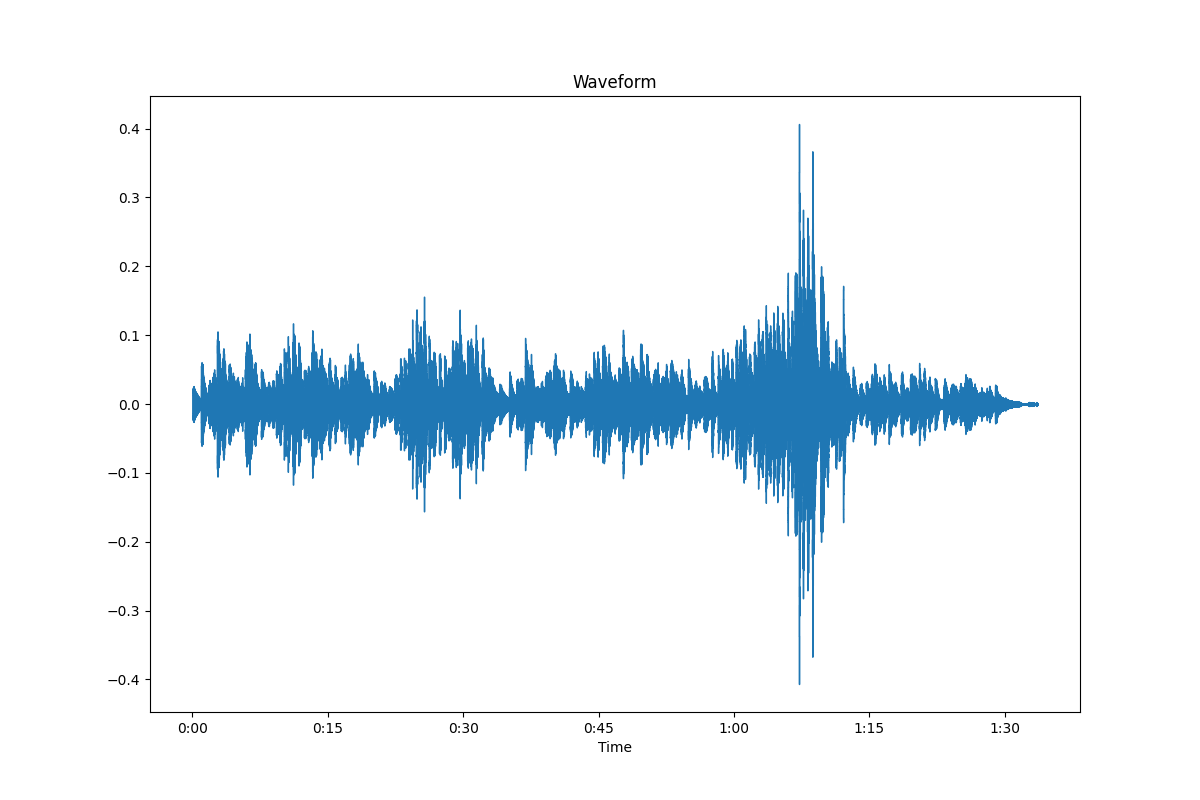
\includegraphics[width=0.8\textwidth]{figures/AudioVisualizations/Waveform.png}
  \caption{Example of an audio waveform.}
  \label{fig:waveform}
\end{figure}

To represent the three signal dimensions, the plot needs to encode time, frequency, and amplitude or energy. The spectrogram achieves this by placing frequency on the y-axis, time on the x-axis, and using colour to encode amplitude or energy. In this thesis, we use the Mel spectrogram, which organises frequencies according to the Mel scale, a perceptual scale designed to reflect how human listeners judge pitch distances. This representation is particularly relevant to music analysis and is used in the LayerIt demonstration.

\begin{figure}[H]
  \centering
  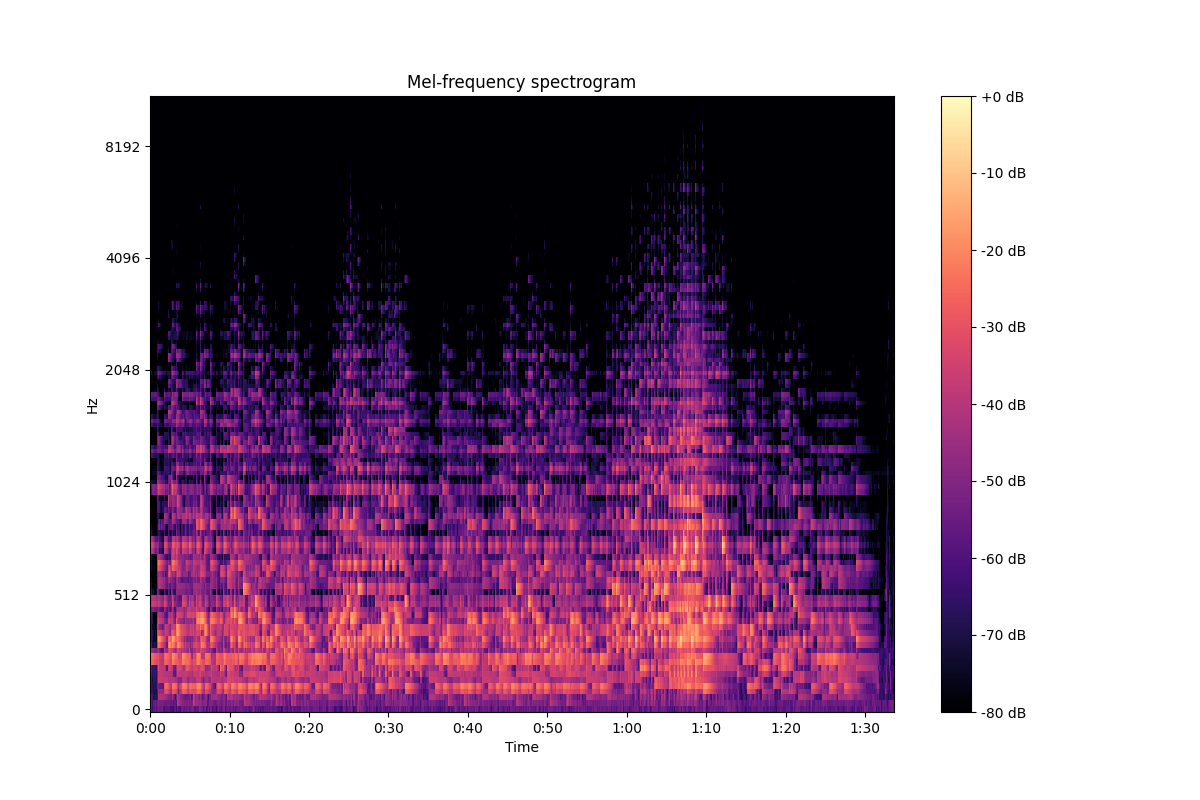
\includegraphics[width=0.8\textwidth]{figures/AudioVisualizations/SpectogramMel.png}
  \caption{Example of Mel spectrogram.}
  \label{fig:spectrogram_mel}
\end{figure}

The Constant-Q Transform (CQT) and chromagram are visual representations that derive from the spectrogram. Whereas a spectrogram shows frequency data, the CQT and chromagram can be used to visualise note-related information: tone height in the case of the CQT and chroma in the case of the chromagram. The following quote explains these terms:
\begin{quotation}
``(...) a pitch can be separated into two components, which are referred to as tone height and chroma. The tone height refers to the octave number and the chroma to the respective pitch spelling attribute contained in the set \{{C, C$\sharp$, D,(...), B}\}.''
\cite{mullerFundamentalsMusicProcessing2015}
\end{quotation}

The CQT organises its frequency content using geometrically spaced frequency bins. This is done to resemble the equal-tempered system.

\begin{figure}[H]
  \centering
  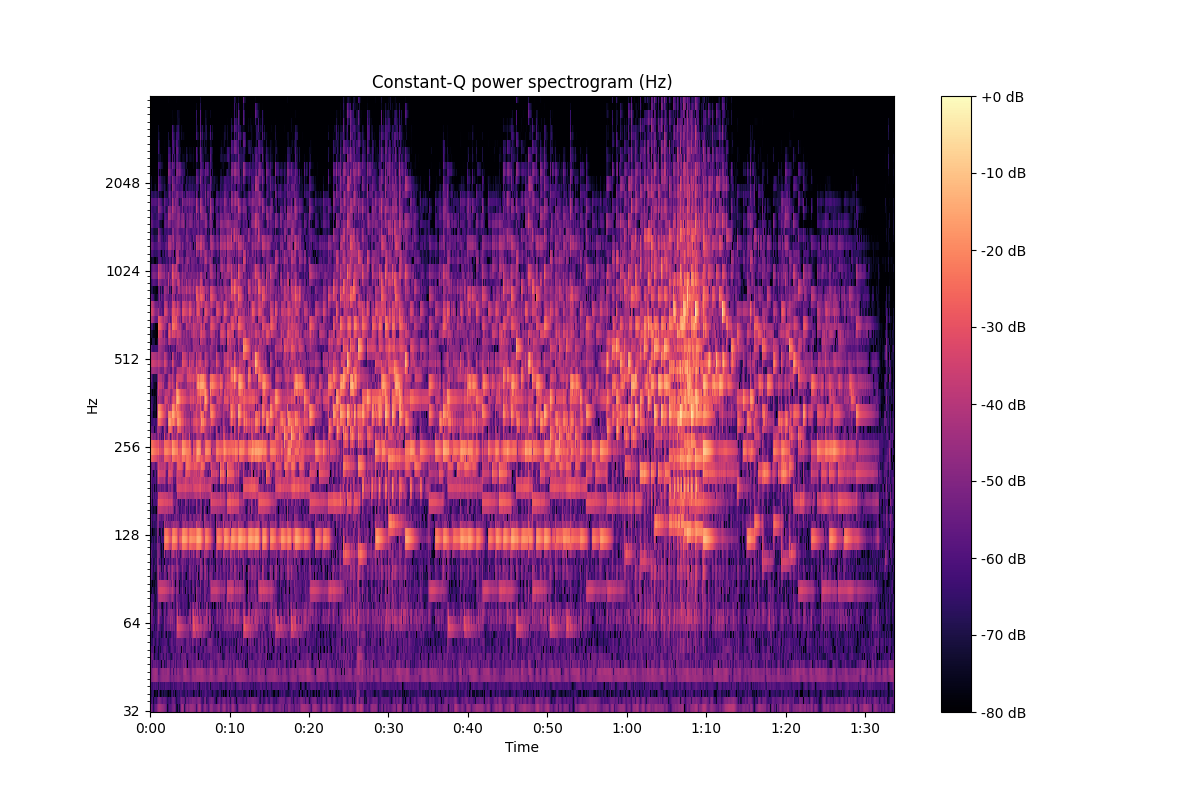
\includegraphics[width=0.8\textwidth]{figures/AudioVisualizations/SpectogramCQT.png}
  \caption{Example of a CQT.}
  \label{fig:spectrogram_cqt}
\end{figure}

While the CQT can distil the frequency spectrum into bins that correlate with individual notes, the chromagram takes this a step further by visually summing the energy of each note across all octaves. Thus, in the end, we obtain a plot divided into 12 lines, each representing a given note. In its essence, this type of visualisation shows the use of the same notes across the recording. A chromagram can be useful for determining harmonic and scale-related information.

\begin{figure}[H]
  \centering
  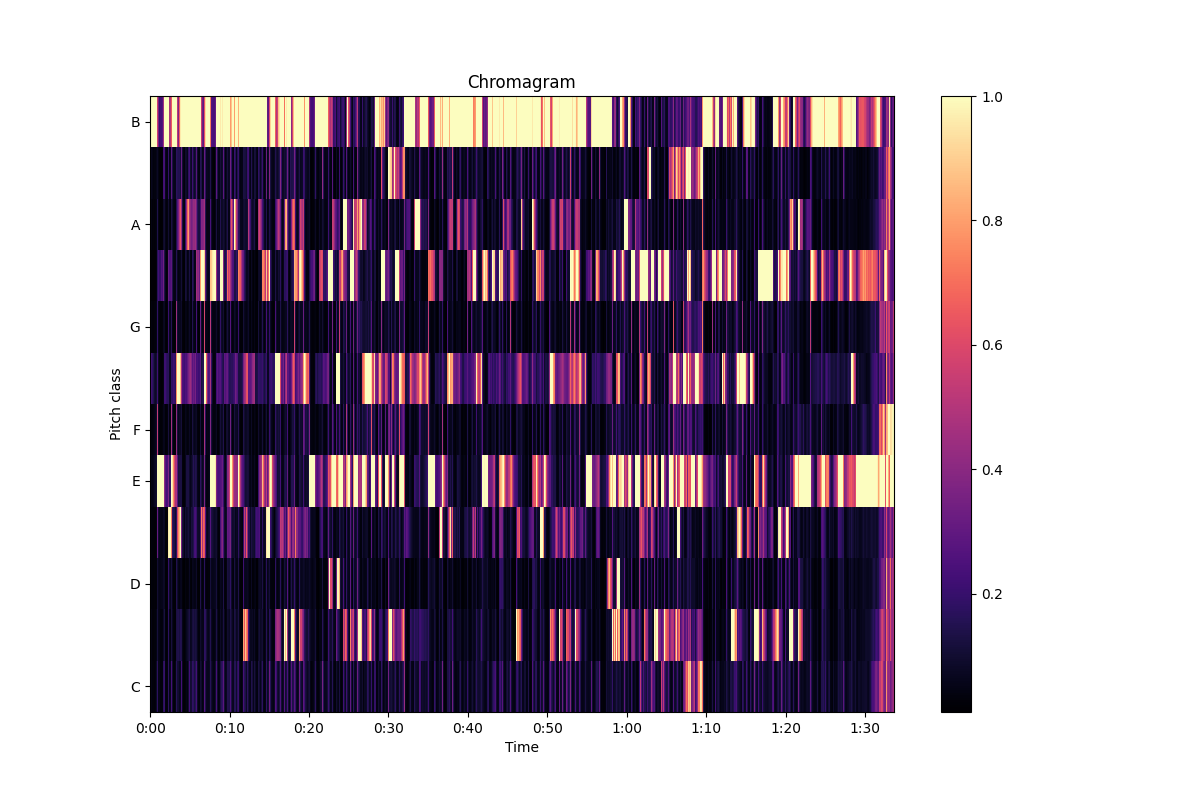
\includegraphics[width=0.8\textwidth]{figures/AudioVisualizations/Chromagram.png}
  \caption{Example of a chromagram.}
  \label{fig:Chromagram}
\end{figure}

\cite{mullerFundamentalsMusicProcessing2015, jungUnifiedCrossmodalTranslation2026a, khodzhaevPracticalGuideSpectrogram}

\section{MIR Visualisation Tools}\label{sec:dialecto}
Within MIR, visualisation workflows typically fall into two broad categories: GUI-based tools and programming-based workflows. Together, these workflows address complementary needs, ranging from interactive inspection and annotation to custom analysis and visual composition. GUI-based tools emphasise direct exploration, while programming-based workflows enable greater control, customisation, and reproducibility. Within this landscape, LayerIt is positioned as a framework for the reproducible composition of score-aligned visualisations.

Sonic Visualiser \cite{cannam2010SonicVisualiserOpen} is an open-source desktop application for the analysis, visualisation, and annotation of audio recordings, particularly music recordings. It provides standard visualisation facilities and supports plugins for automated analysis methods, allowing users to inspect audio and visualise computational outputs. These capabilities make it useful for general audio analysis as well as for the development and interpretation of MIR methods. Its open-source distribution also supports the adaptation and extension of the application to meet specialised research needs, making it a relevant baseline for research-oriented visual work.

A particularly relevant example is Piano Precision, a Sonic Visualiser fork that is a GUI for visualising score-aligned spectrograms. By adapting Sonic Visualiser, Piano Precision extends this workflow with a score view and score-aware annotations. The authors describe this relationship as follows:

\begin{quotation}
``The Piano Precision UI is adapted from Sonic Visualizer, with an additional area displaying a score (...) The interface is designed to help streamline the processes of loading a digital score and a performance recording, editing and visualising annotations (...), and exporting score-aware annotations.''\cite{jiangPIANOPRECISIONADVANCING2025}
\end{quotation}

This makes Piano Precision particularly relevant to research involving correspondence between a performance and its score. Its main strength is the integration of interactive navigation and score-aware annotation within a GUI, enabled by extending an open-source audio-analysis environment. To establish this correspondence, Piano Precision uses Piano Aligner, an integrated plugin developed by the same authors that detects onsets in a performance and links them to their corresponding positions in the MEI score. These links allow the interface to synchronise the playback view with the relevant score elements and associate annotations with both modalities.

Specialised MIR research can also require visualisations that combine several data types, such as audio, scores, annotations, and computational outputs, in a layout designed for a specific research question. These combinations are not always available as pre-built views in GUI-based tools. In such cases, programming-based workflows provide a complementary solution. Python libraries such as Librosa and Matplotlib, together with tools such as Jupyter Notebooks, allow researchers to implement custom feature extraction, analysis, and visualisation pipelines. Such workflows can be versioned, shared, and included directly in publications, which supports reproducibility. They also integrate naturally with machine-learning and large-scale data-analysis pipelines. Their flexibility, however, usually means that the researcher must implement the composition logic, data transformations, and alignment-dependent layout themselves.

LayerIt addresses this composition problem. It provides reusable objects for composing score, audio, annotation, and algorithmic layers into a static visualisation. The score-performance alignment is supplied externally, while LayerIt uses that alignment to place the different representations on a shared visual axis and export the result as structured SVG. In this sense, LayerIt combines the customisability and reproducibility of code-based workflows with a framework dedicated to reusable score-aligned visual composition.

\section{Audio-to-score alignment}
Audio-to-score alignment, also referred to as score matching or score alignment, consists of synchronizing an audio recording of a musical performance with its corresponding symbolic score \cite{carabias-ortiAUDIOSCOREALIGNMENTa}. In practical terms, the goal is to establish correspondences between what is heard in the recording and what is represented in the score, enabling tasks such as score following, guided listening, interactive navigation between audio and score, and research-oriented analysis.

Time To Align! distinguishes graphical, logical, and physical temporal domains and provides a general model for recording alignments among them \cite{hentschelTimeAlignModelling2026}. In this model, an alignment is a reusable artefact that records correspondences and their provenance across timelines. LayerIt addresses a complementary problem: it uses an available score-performance alignment to compose graphical, symbolic, and audio-derived representations into a shared score-aligned visualisation.

For the purposes of this thesis, it is useful to distinguish between \textbf{physical time} and \textbf{abstract time}. Physical time refers to positions in the performance, such as the duration of the audio recording, samples or frames used by audio features, detected beat times, and model activation probabilities. Abstract time refers to positions in the musical structure represented by the score, such as notes, beats, measures, and other metrical or structural locations. The alignment step maps positions in abstract score time onto positions in the physical performance time. LayerIt then uses this mapping to place score material and other representations on a common visual axis; it does not compute the mapping itself.

The purpose of an alignment is not limited to algorithmic matching. Thomas et al. \cite{thomasLinkingSheetMusic2012} describe score--audio linking structures as a basis for accessing and exploring multimodal music sources within a single framework. LayerIt uses an available linking structure for a more specific purpose: the generation of static, score-aligned visualisations. It does not compute the alignment itself. Existing synchronisation toolkits, such as Sync Toolbox, provide dynamic-time-warping-based pipelines that could supply an upstream alignment in future work \cite{mullerSyncToolbox2021}.

In the literature, it is useful to distinguish between two broad alignment strategies. The first is \textbf{time-warped alignment}, in which the score is mapped onto a continuous performance timeline \cite{goeblLetsScoreWarpAgain2025a}. This approach preserves a direct temporal relationship between score elements and audio playback, and it is especially relevant when every relevant musical event needs to be placed along the time axis. The second is \textbf{link-based alignment}, in which the relationship between score and performance is established through discrete anchor correspondences \cite{jiangPIANOPRECISIONADVANCING2025}. Rather than continuously warping the score, this approach links selected score positions to performance positions and uses those reference points to organize the alignment \cite{weigl2020MultimodalMusicInformation}.

These two strategies are not separate tasks so much as different ways of representing the same underlying correspondence problem, and the distinction becomes important for the rest of this thesis. Time-warped alignment is the more continuous formulation, while link-based alignment is the more anchor-driven formulation. This terminology will be used throughout the following chapters.

Alignment systems can also be classified by when the matching is performed. \textbf{Offline alignment} processes a complete recording after the performance has finished. Because it can access the full signal, offline alignment can use future information to determine the best possible correspondence, which makes it suitable for analysis, annotation, and audio editing. \textbf{Online alignment}, also known as score following, performs the matching in real time while the audio is being received. Since it cannot rely on future information in the same way, online alignment typically has to trade off latency against precision.

Beyond this temporal distinction, alignments may be carried out at different levels of granularity. The three most common are \textbf{note-level}, \textbf{beat-level}, and \textbf{segment-level} alignment.

\textbf{Note-level} alignments are score matching processes that aim to synchronise at the individual note level. At its core, note-level alignment is based on note and onset/offset detection. In MIR literature it can also be referred to as ``fine-grained alignment'' because of the precision it requires. Contemporary audio-to-score alignment research focuses on this type of alignment not only because of its precision but also because it can retrieve data relevant to other MIR fields and tasks. However, pure note-level alignments might falter if the performance deviates from the score, for example if the performer skips, repeats, or adds notes or score sections. Repeats and jumps are a well-established source of difficulty in score-performance synchronisation \cite{fremereyHandlingRepeats2010}. For this reason, some score-matching solutions combine fine-grained alignment with other methods.

Piano Precision is an example of an application of a link-based note-level score-alignment method. While the recording is playing Piano Precision shows a spectrogram and waveform that follow along a conventional playback cursor while, on a side window that contains the score, highlighting the corresponding elements being played in the score, note by note. This enables annotations to be mapped to both the audio and individual score elements simultaneously. The authors note the usefulness of this tool for performance researchers \cite{jiangPIANOPRECISIONADVANCING2025} however, we will make the case that such feature is useful for BT and MIR research more broadly.

\textbf{Beat-Level} alignments aim to follow along beat and/or measures dictated in the score, and then linking them to the performance. Early score aligners \cite{duanSoundprismOnlineSystem2011} would rely on such methods. Today, score alignment solutions, although mostly are note-level types, still combine Beat-Level alignment layers within their algorithms. A good example of this comes from \cite{peterAutomaticNoteLevelScoretoPerformance2023}, in it the authors improved on other alignment models, one strategy employed was adding analysis of ``alignments at both the beat and the bar level''. The beat level alignment would serve as ``anchor points'' in order to prevent ``cascading errors, as misalignment will not propagate beyond the next anchor point'', they noted that this improved results of automatic alignments.

\textbf{Segment} type alignments, map broad portions of performance audio to corresponding visual blocks in the score. This type of score matching is mostly made manually, it is common to see it in follow-along videos to help viewers listen to the music while visualising the score. This type of alignment is considered ``weak but musically meaningful'' \cite{jungUnifiedCrossmodalTranslation2026a} since segments can be deliberately chosen i.e., to better show melodic or harmonic structure.

Among the visual alignment tools relevant to this thesis, ScoreWarp is especially important. ScoreWarp presents a score on a physical time axis, shifting each musical element so that its visual position corresponds to the time at which it sounds \cite{goeblLetsScoreWarpAgain2025a}. In other words, it implements a time-warped visualisation that maps abstract score time onto physical performance time while preserving the semantic structure of the original MEI data. This makes ScoreWarp a strong example of how alignment can be used not only as an algorithmic task, but also as a visual framework for interacting with music information. In the next chapter, we will return to this tool in more detail, since it became one of the key references for the development of this thesis.

\section{Summary}
This chapter provided a comprehensive overview of MIR visualisation techniques and tools, establishing the foundation for understanding audio-to-score alignment. 

We began by categorising music visualisations into three main types: traditional sheet music representations, symbolic machine-readable formats, and audio-based representations. This established the importance of MEI and Verovio, as well as the use of SVG in this context.

We then examined the contemporary landscape of MIR visualisation tools, distinguishing between GUI-based solutions such as Sonic Visualiser and Piano Precision, which provide user interfaces for audio analysis, and code-based workflows that afford researchers greater flexibility to develop specialised visualisations tailored to specific research questions. Python-based approaches using libraries such as Librosa and Matplotlib have become widely used in MIR research, particularly because of their integration with machine-learning pipelines and reproducibility requirements.

Finally, we introduced one of the core tasks of this thesis: audio-to-score alignment. This process synchronizes musical performances with their corresponding symbolic scores. ScoreWarp emerged as a particularly relevant tool, demonstrating how MEI and Verovio can be leveraged to create visually warped scores that maintain semantic integrity while aligning with performance time.